\input ../SlidePreamble
\input ../preamble


\begin{document}

{\Huge
  \centerline{\bf TTIC 31230,  Fundamentals of Deep Learning}
  \vfill
  \centerline{David McAllester, Autumn   2022}
  \vfill
  \centerline{\bf Contrastive Coding}
  \vfill
  \vfill


\slide{Contrastive Coding for Speech}
\centerline{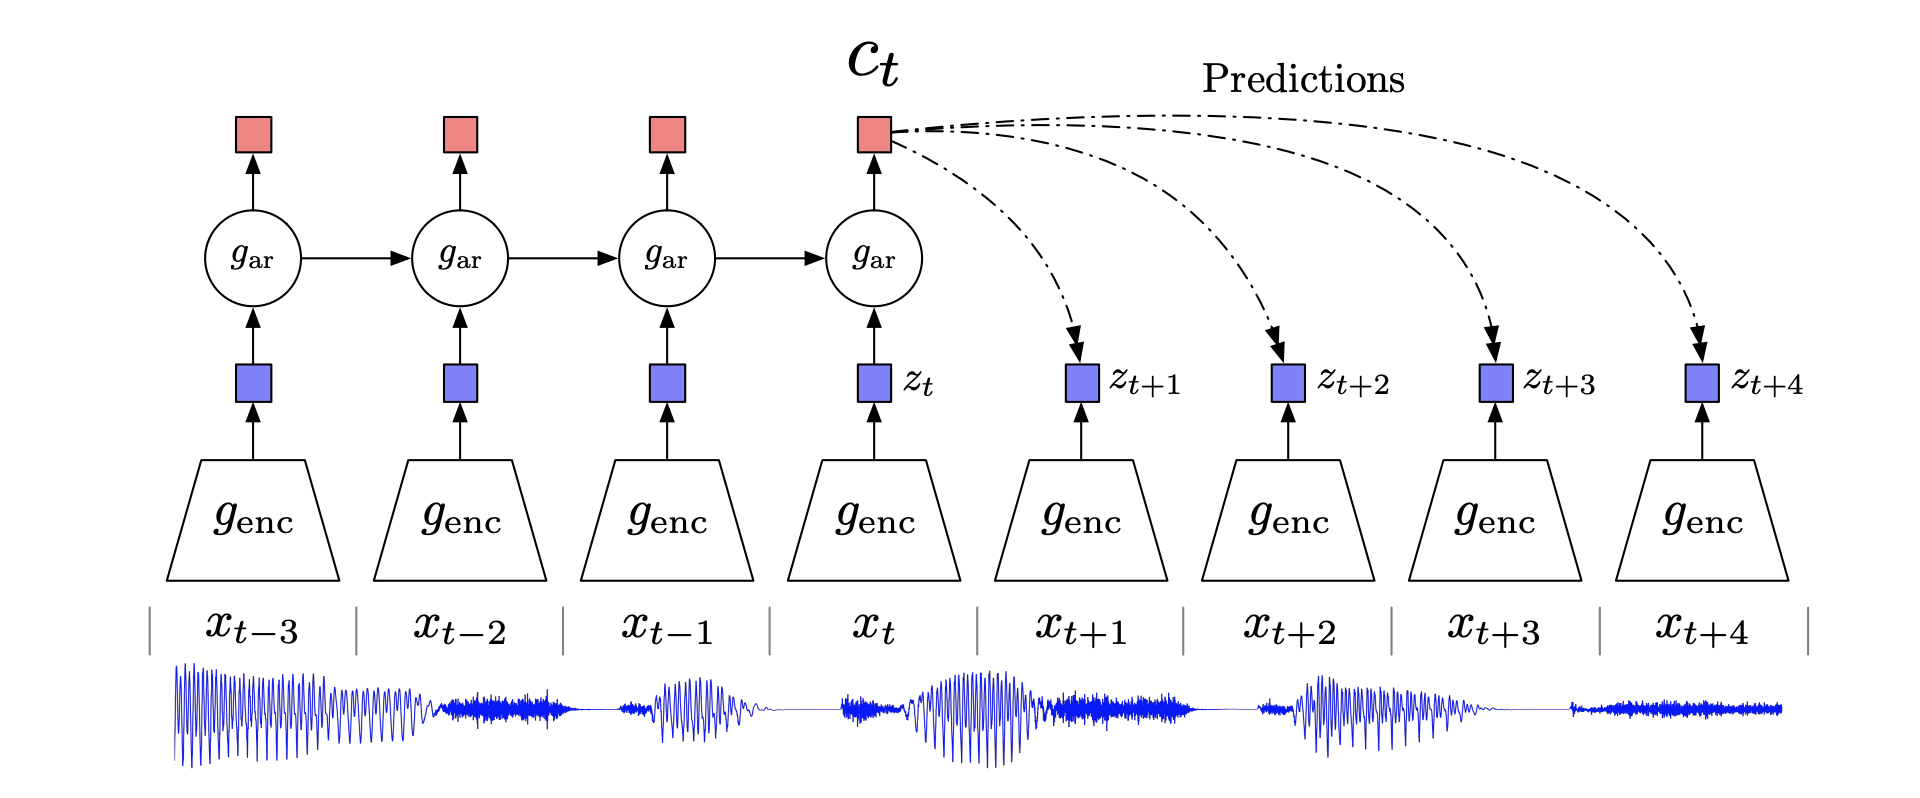
\includegraphics[width = 6 in]{\images/CPC}}
\centerline{\huge van den ORD et al. 2018}

\vfill
Consider the problem of learning phonetic representations of speech sounds.  In the figure each $z_t$ is a symbol representing the sound at time $t$.


\slide{Contrastive Coding for Speech}
\centerline{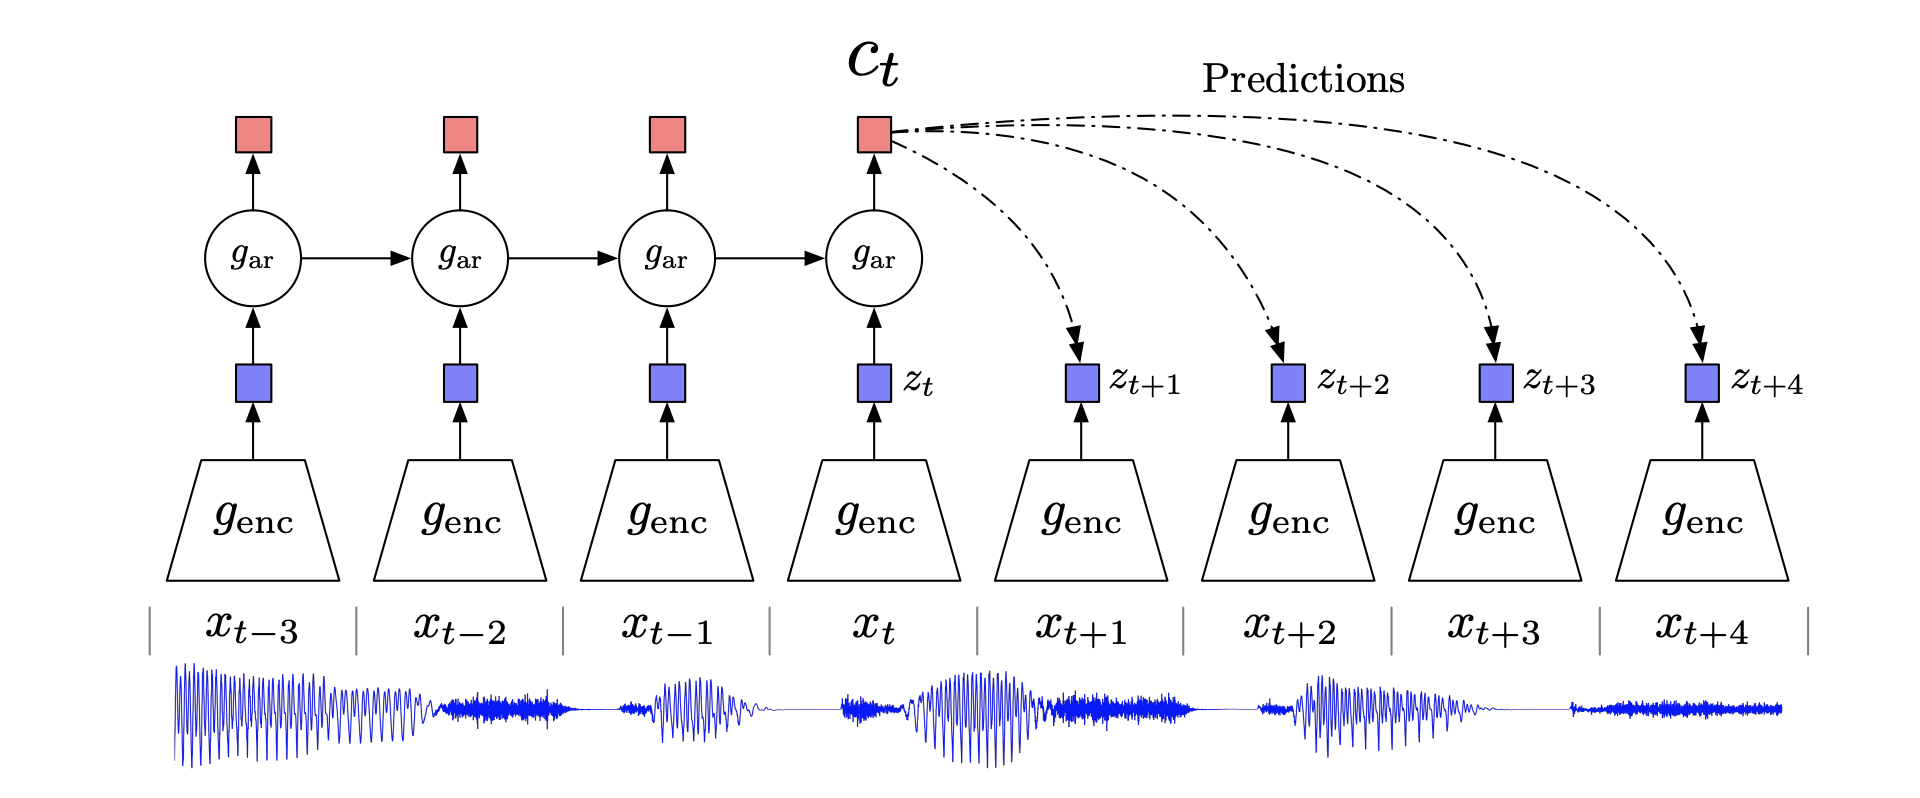
\includegraphics[width = 6 in]{\images/CPC}}
\centerline{\huge van den ORD et al. 2018}

\vfill
Here we want to train the networks so as to capture the mutual information between $x_1,\ldots,x_t$ and $x_{t+i}$.

\slide{Contrastive Coding for Speech}
\centerline{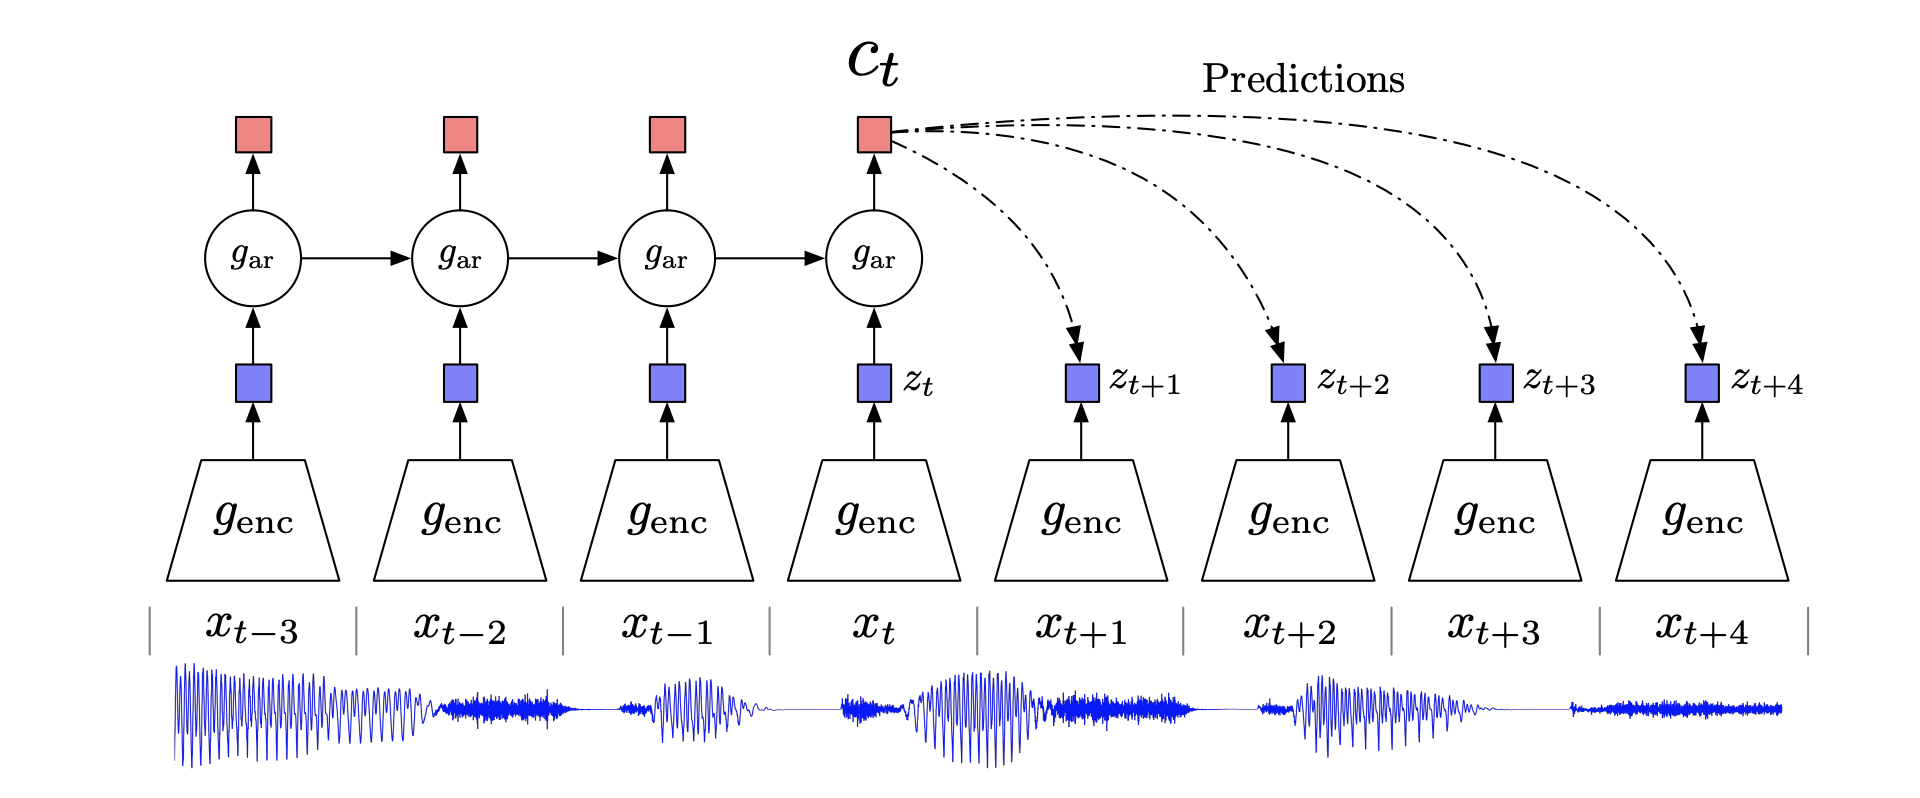
\includegraphics[width = 6 in]{\images/CPC}}
\centerline{\huge van den ORD et al. 2018}

\vfill
{\bf Unlike VAEs}, contrastive coding is about {\bf capturing mutual information}. There is no attempt to model the input speech sound.
Intuitively we want to {\bf separate signal from noise} and avoid modeling noise.

\slide{Contrastive Coding for Speech}
\centerline{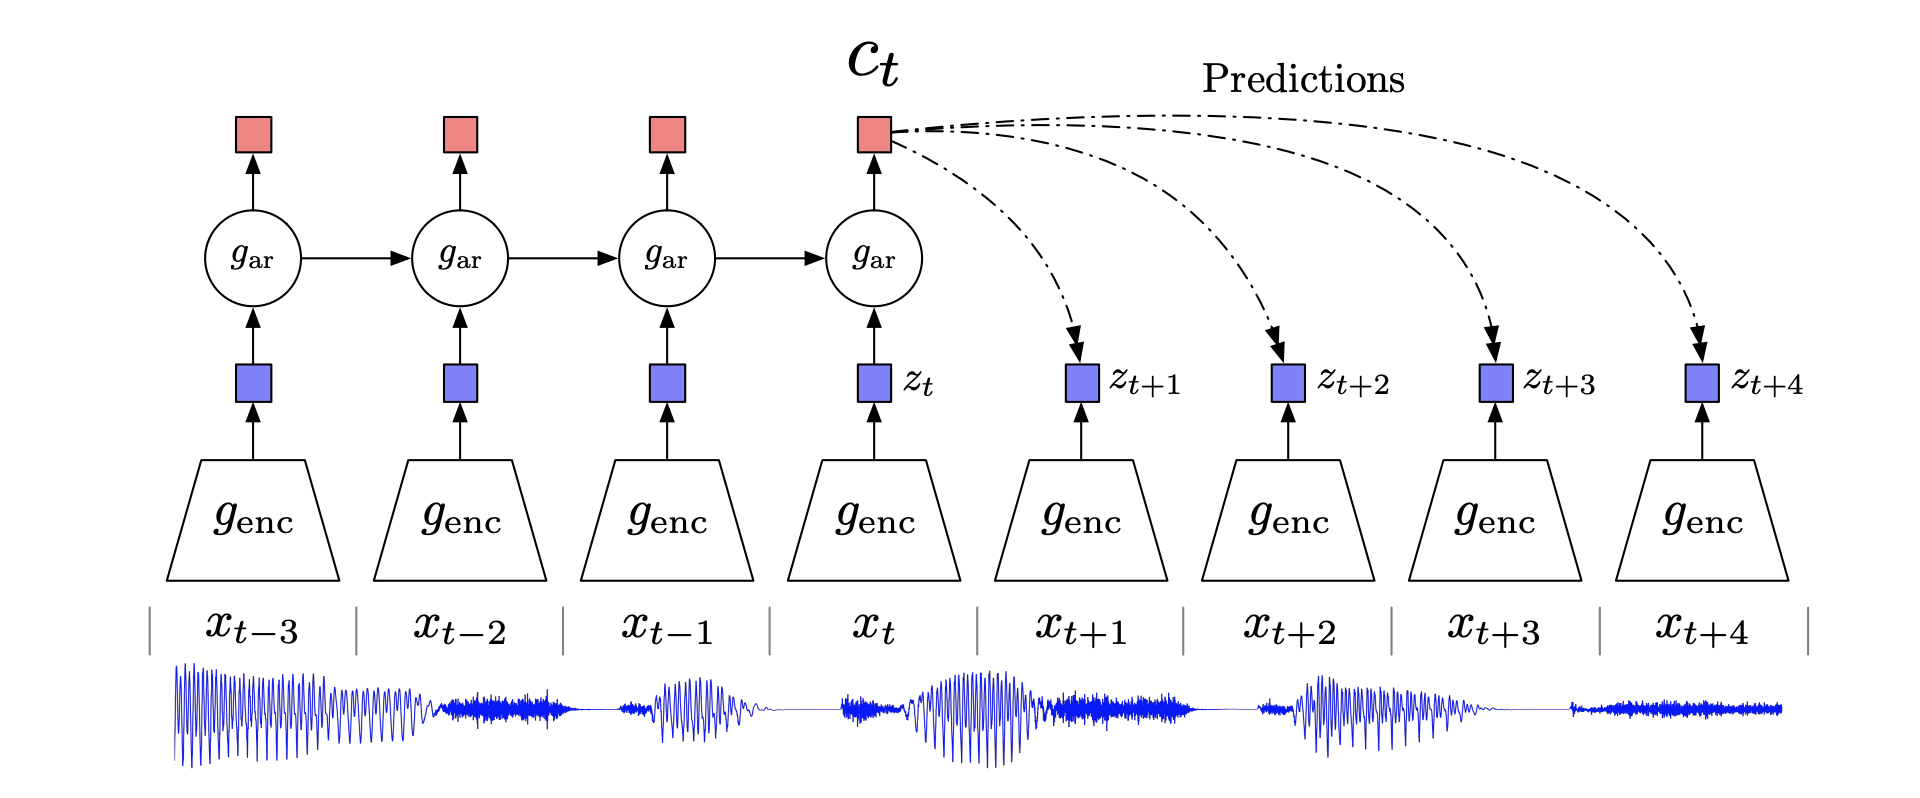
\includegraphics[width = 6 in]{\images/CPC}}
\centerline{\huge van den ORD et al. 2018}

\vfill
Here we want to train the networks so as to capture the mutual information between $x_1,\ldots,x_t$ and $x_{t+i}$.

\vfill
We abstract this problem to that of capturing the mutual information between any two arbitrary random variables $x$ and $y$.

\slide{Wav2vec 2.0, June 2020, Facebook}

\vfill
Trained on 53k hours of unlabeled audio (no text) they convert speech to a sequence of discrete quantized vectors they call ``pseudo-text units''.

\vfill
By training on only one hour of human-transcribed audio, and using the Wav2vec transcription into pseudo-text, they outperform the previous state of the
art in word error rate for 100 hours of human-transcribed text.

\slide{GLSM, February 2021, Facebook}

Generative Spoken Language Model (GSLM)

\vfill
They then train a generative model of the sequences of pseudo-text units learned from unlabeled audio.


\vfill
This model can continue speech from a speech prompt in much the same way that GPT-3 continues text from a text prompt.

\vfill
Semantic and grammatical structure in a ``unit language model'' is recovered
from speech alone.


\slide{Contrastive Coding}

We draw a batch of pairs $(x_1,y_1), \ldots (x_B,y_B)$ from the population.
For example $x$ is the speech signal up to time $t$ and $y$ is the speech signal
at $t+i$.

\vfill
We then select $b$ uniformly from $1$ to $B$ and construct the tuple $(x_b,y_1,\ldots,y_B,b)$.

\slide{Contrastive Coding}

We draw pairs $(x_1,y_1), \ldots (x_B,y_B)$ from the population.
We then select $b$ uniformly from $1$ to $B$ and construct the tuple $(x_b,y_1,\ldots,y_B,b)$.

\vfill
We then train a model to predict $b$.
\vfill
{\huge
\begin{eqnarray*}
\enc_x^*,\enc_y^* & = & \argmin_{\enc_x,\enc_y} \;E_{(x,y_1,\ldots,y_B,b)}\left[-\ln P_{\enc_x,\enc_y}(b|x,y_1,\ldots,y_B)\right]
\end{eqnarray*}

\begin{eqnarray*}
P_{\enc_x,\enc_y}(b|x,y_1,\ldots,y_B) & = & \softmax_b\; \enc_x(x)^\top\enc_y(y_b)
\end{eqnarray*}
}

\slide{The Contrastive Coding Theorem}

For any distribution on pairs $(x,y)$, with contrastive probabilities computed by

\begin{eqnarray*}
P(b|x,y_1,\ldots,y_B) & = & \softmax_b\;s(x,y_b)
\end{eqnarray*}

we have

{\huge
\begin{eqnarray*}
I(x,y) & \geq & \ln B - \;\;E_{(x,y_1,\ldots,y_B,b)}\left[-\ln P(b|(x,y_1,\ldots,y_B))\right]
\end{eqnarray*}
}

Chen et al., On Variational Bounds of Mutual Information, May 2019.

\slide{Augmentation Contrastive Coding for Images (SimCLR)}

(SimCLR:) A Simple Framework for Contrastive Learning of Visual Representations, Chen et al., Feb. 2020 (self-supervised leader as of February, 2020).

\vfill
They construct a distribution on pairs $\tuple{x,y}$ defined by drawing an image from ImageNet and then drawing $x$ and $y$ as random ``augmentations'' of the image.

\vfill
Augmentations include (among others) reflections, croppings, and changes in the color map.

\slide{Augmentation Contrastive Coding for Images (SimCLR)}

\vfill
They drawing an image from ImageNet and then draw $x$ and $y$ as random augmentations
of the same image.

\vfill
They then train a single coding function $\enc$ that applies to any augmentation and train the ecoding function by the
the contrastive coding objective objective.

\begin{eqnarray*}
\enc^* & = & \argmin_\enc \;E_{(x,y_1,\ldots,y_B,b)}\left[-\ln P_\enc(b|(x,y_1,\ldots,y_B)\right]
\end{eqnarray*}

\begin{eqnarray*}
P_\enc(b|x,y_1,\ldots,y_B) & = & \softmax_b\; \enc(x)^\top \enc(y_b)
\end{eqnarray*}


\slide{Augmentation Contrastive Coding for Images (SimCLR}

The encoder is then used on images to define a feature vector for images.

\vfill
They then train a {\bf linear} imagenet classifier on the feature map defined by the encoder.

\vfill
This is called linear probing.

\slide{Augmentation Contrastive Coding for Images (SimCLR)}

\centerline{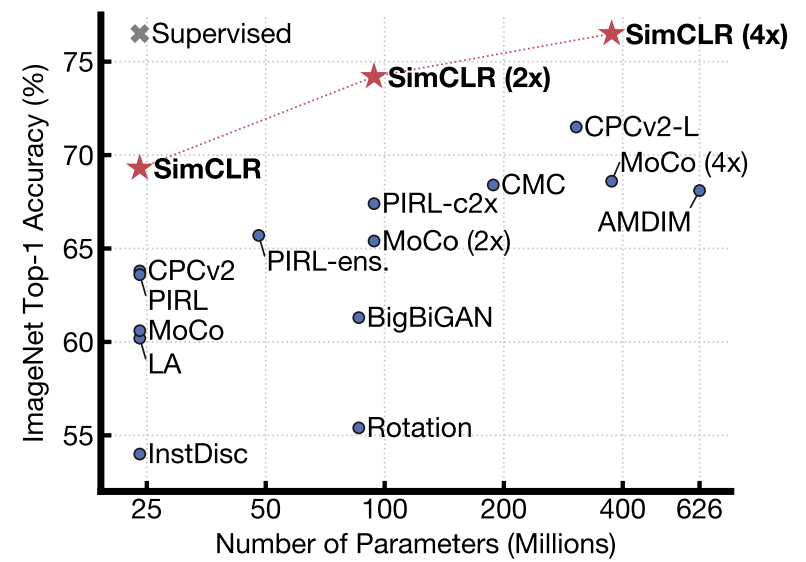
\includegraphics[height=3.5 in]{\images/SimCLR}}

\vfill
\centerline{\huge Chen et al. 2020}

\slide{CLIP, January 2021, OpenAI}

CLIP: Contrastive Language-Image Pre-training.

\vfill
Trained on images and associated text (such as image captions or hypertext links to images) CLIP computes embeddings of text and embeddings of images
(``co-embeddings'') trained to capture the mutual information between the two.

\vfill
This is done with contrastive coding.

\slide{Contrastive Coding}


Consider a population distribution on pairs $\tuple{x,y}$ (such as images and associated text).

\vfill
We are interested in finding embedding functions $\enc_x$ and $\enc_y$ such that $\enc_x(x)$ and $\enc_y(y)$ are in the same embedding space
and capture the mutual information between $x$ and $y$.

\slide{CLIP Constrastive Coding}

\centerline{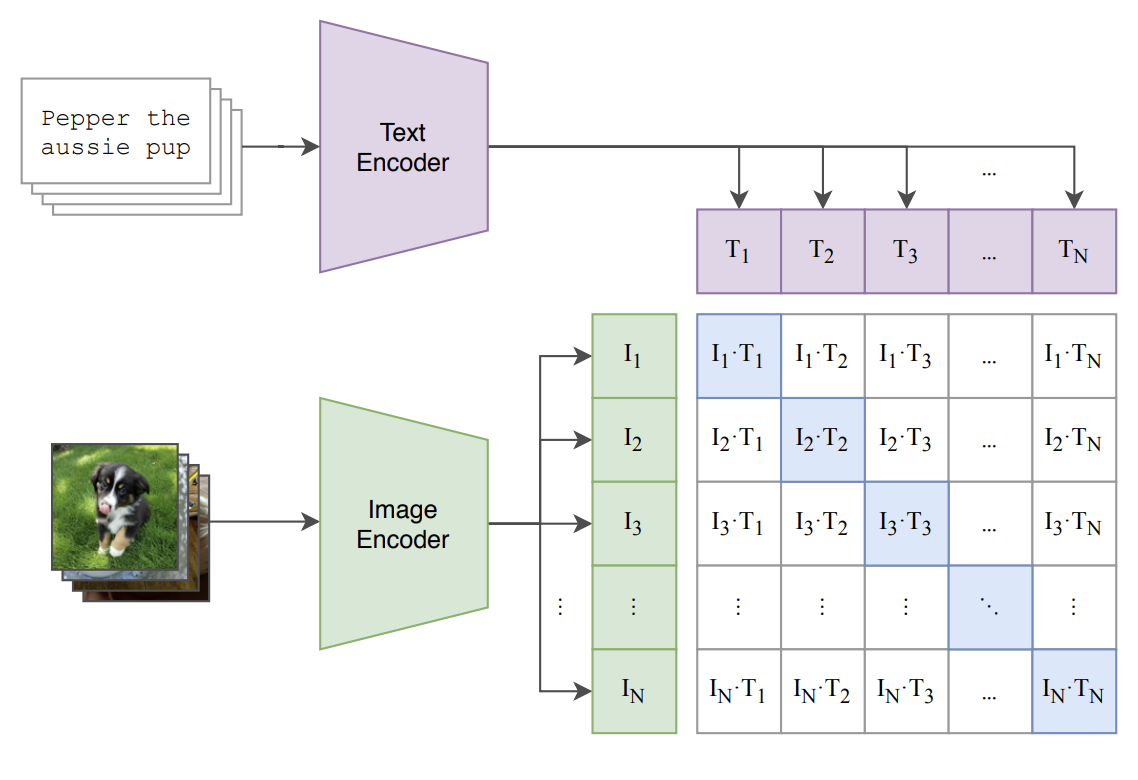
\includegraphics[height= 5in]{\images/CLIPTraining}}

\slide{The Contrastive Coding Theorem}

\begin{eqnarray*}
I(x,y) & \geq & \ln B - \;\;E_{(x,y_1,\ldots,y_B,b)}\left[-\ln P(b|(x,y_1,\ldots,y_B)\right]
\end{eqnarray*}

\vfill
For CLIP the batch size $B = 2^{15}$ so we can potentially guarantee 15 bits of mutual information.

\slide{CLIP Image Classification}

\centerline{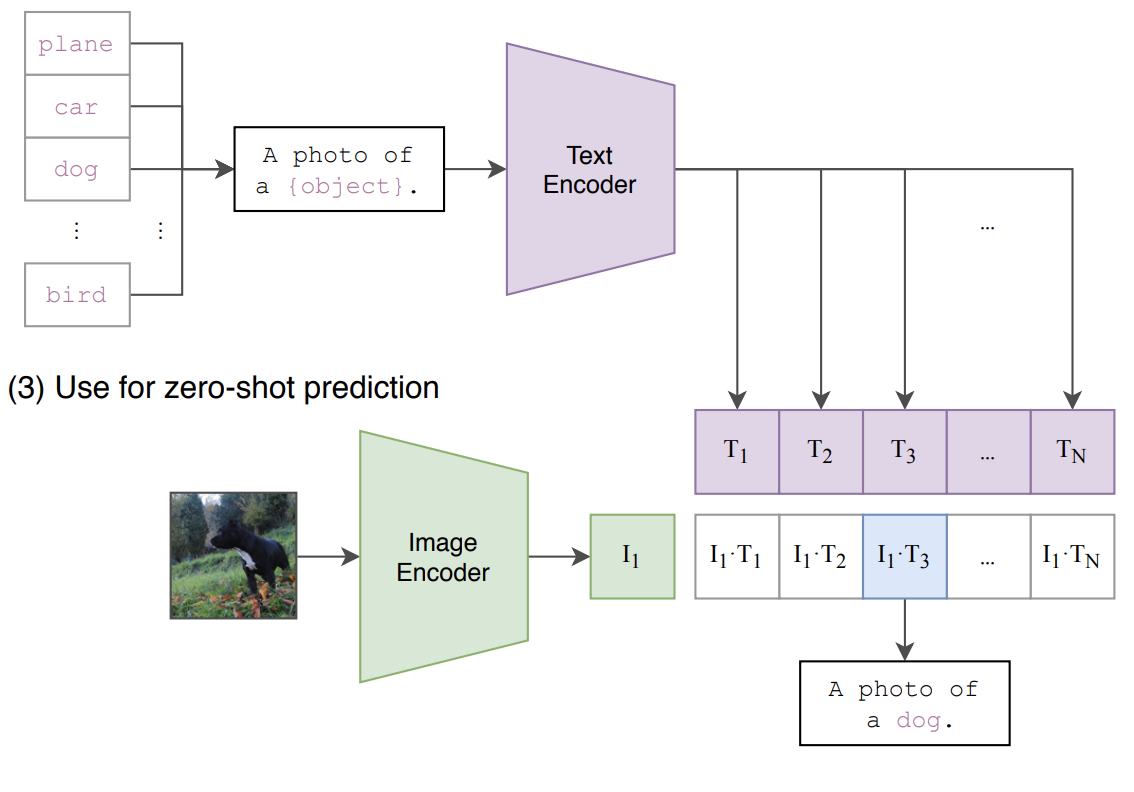
\includegraphics[height= 5in]{\images/CLIPClassifier}}

\slide{Zero-Shot Image Classification}

\centerline{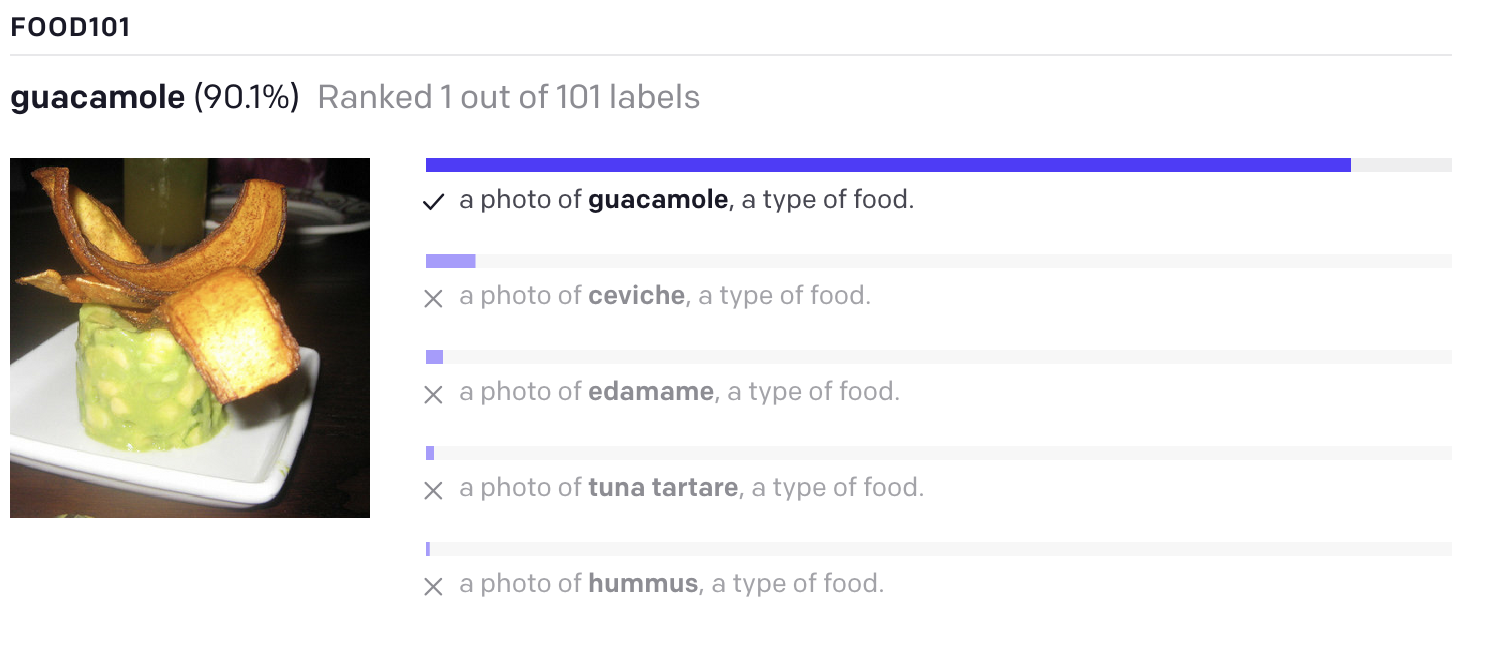
\includegraphics[width = 7in]{\images/CLIP0}}

\slide{Zero-Shot Image Classification}

\centerline{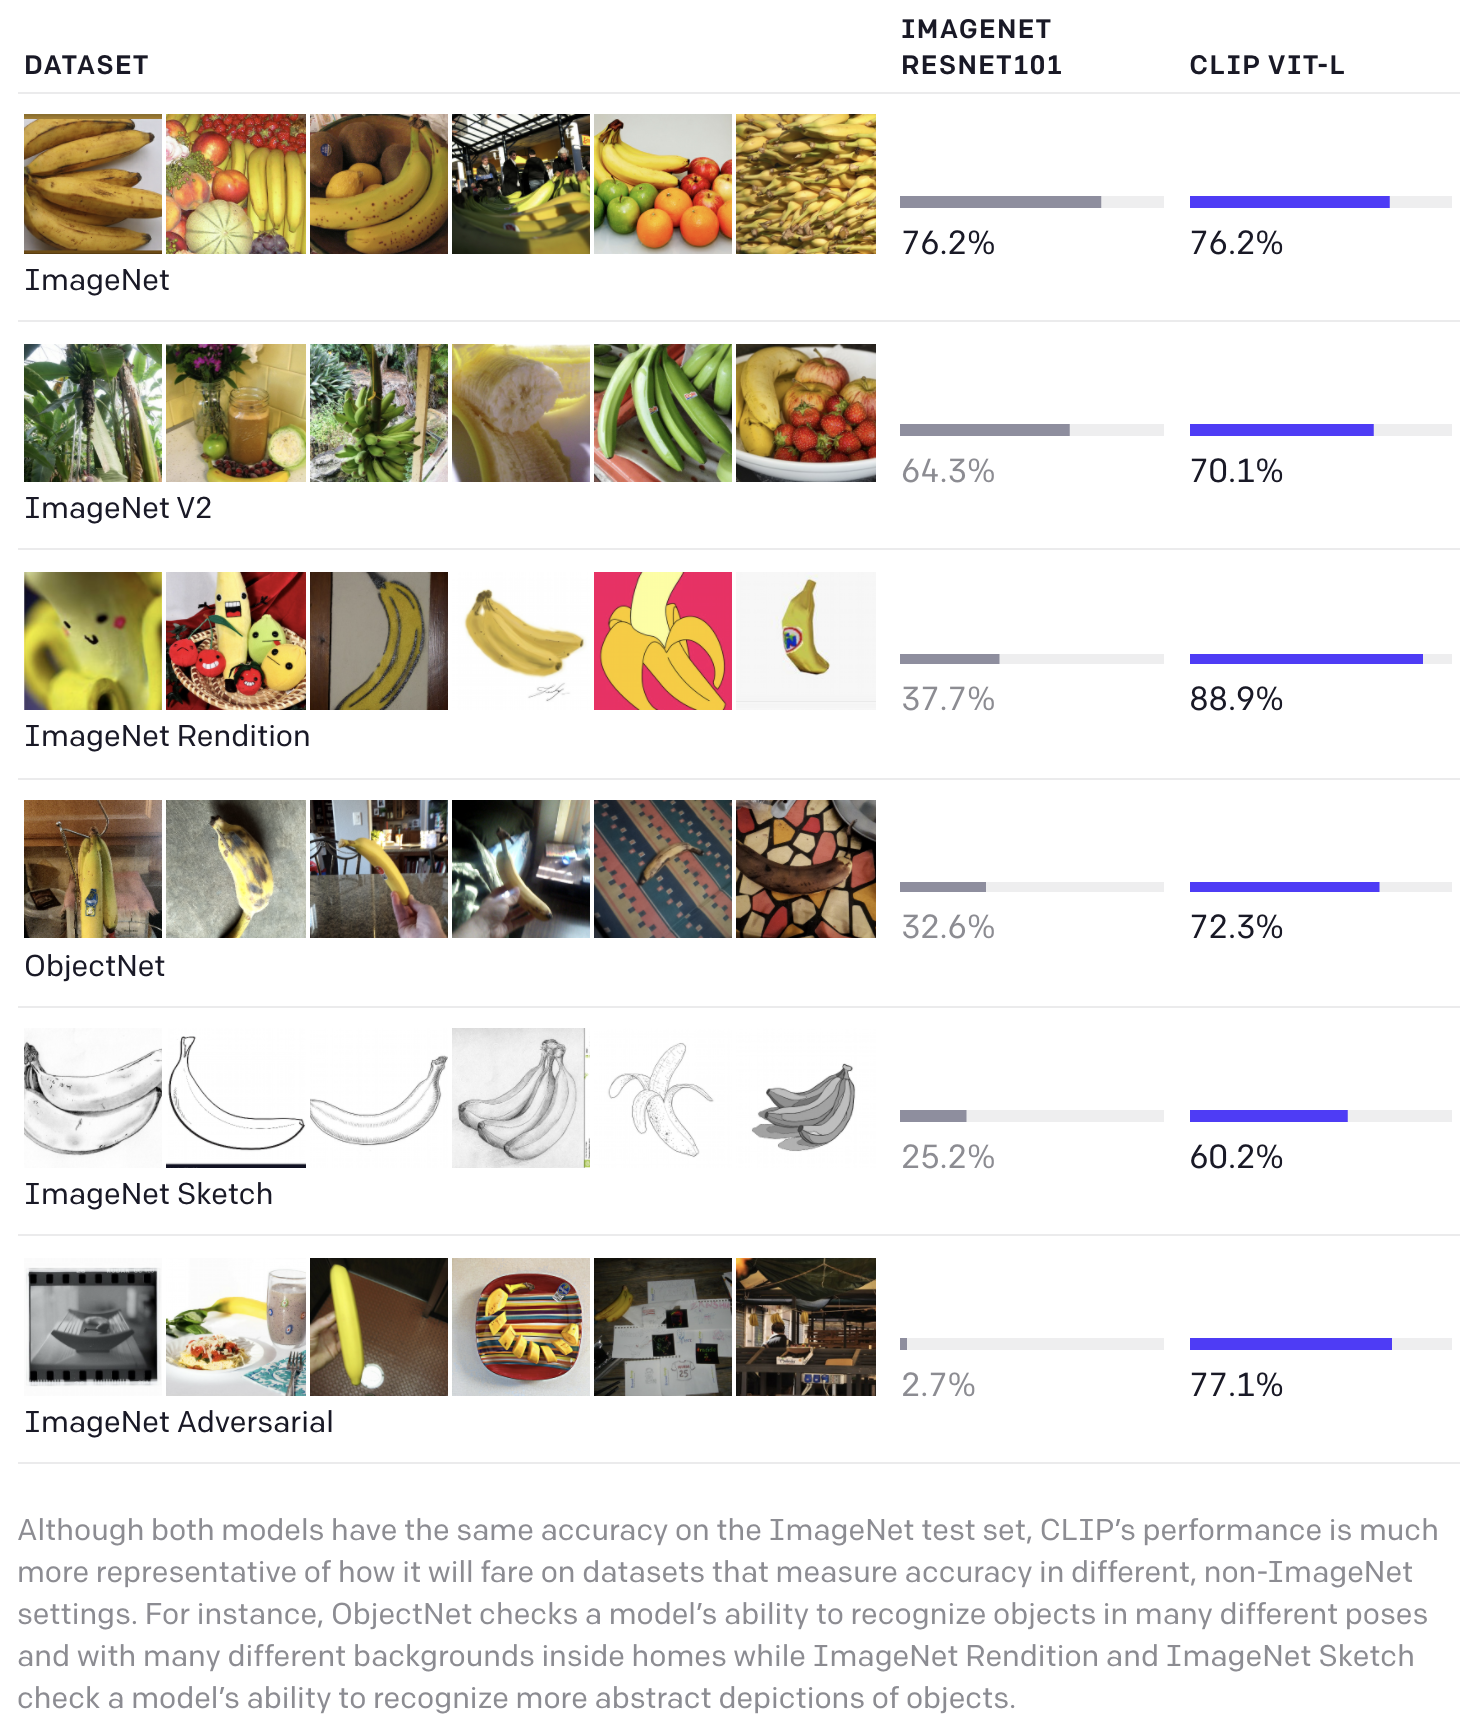
\includegraphics[height= 5in]{\images/CLIP1}}

\slide{A Weakness of Contrastive Coding}

{\huge
\begin{eqnarray*}
I(x,y) & \geq & \ln B - \;\;E_{(x,y_1,\ldots,y_B,b)}\left[-\ln P(b|(x,y_1,\ldots,y_B)\right]
\end{eqnarray*}
}

The discrimination problem may be too easy.

\vfill
The guarantee can never be stronger than $\ln B$ where $B$ is the batch size.

\vfill
Suppose we have 100 bits of mutual information as seem plausible for translation pairs.

\slide{A possibly Better Estimate of Mutual Information}

We might be able to get a better estimate of the mutual information using

$$I(x,y) \geq I(\enc(x),y) = H(\enc(x)) - H(\enc(x)|y)$$

\vfill
and estimating $H(\enc(x))$ and $H(\enc(x)|y)$ separately.

\vfill
For this to be meaningful it seems best to use a discrete code $\enc(x)$ such as might be achieved with $K$-means clustering.

\vfill
We upper bound $H(\enc(x)|y)$ by a cross entropy model and estimate (but not lower bound) $H(\enc(z))$
by a cross entropy model.

\slide{END}

}
\end{document}

